\chapter{Discussion}\label{chap:discussion}

In Chapter~\ref{chap:implementation} we present our formalisation of
infinitary term rewriting and in the current chapter we discuss some
aspects of it. First, the representation we use for rewrite sequences
is motivated and the resulting definitions are related to the notion
of convergence. We then comment on some technicalities in the
implementation. Finally, we conclude with an evaluation of our
formalisation.


\section{Representing Rewrite Sequences}

% TODO: leave out ', with the appropriate conditions...' ?
In Definition~\ref{def:seq}, transfinite rewrite sequences are
introduced as partial functions from ordinals to rewrite steps, with
the appropriate conditions on source and target terms of subsequent
rewrite steps. Could we not translate this directly to \Coq?

% TODO: one problem, and other problem?
A problem with partial functions from ordinals to rewrite steps is that we
would need a decidable order on the ordinals. Consider a non-trivial rewrite
sequence of length $\alpha$. The partial function representing this
rewrite sequence must compare its input value (an ordinal) to all possible
input values (ordinals up to $\alpha$) in order to decide what rewrite step to
produce, in finite time.

The order on our tree ordinals is not decidable (consider comparing the upper
bounds of two infinite sequences). This could be
remedied by using a different representation for the ordinals, for
example axiomatically, as Cantor normal forms, or as sets. We feel
that the inductively defined tree ordinals are a more natural
representation in the constructive type theory of \Coq.

Comparison of ordinals up to some given upper bound may be decidable,
so another remedy for this problem would be to only consider rewrite
sequences of limited length. Motivated by the Compression Lemma, we
could go even further and restrict our representation to rewrite
sequences of length $\le \omega$. This would severely cripple our
formalisation, since much of the theory of infinitary rewriting could
not be developed with this representation (e.g. the Compression Lemma
itself). % and many compressed rewrite sequences are unnatural

Another argument in favour of our representation based on tree
ordinals is that it seems natural for a \Coq formalisation. As a
comparison, lists of finite length are usually defined by induction in
\Coq, not as partial functions from the natural numbers. Our
representation can be seen as a generalisation of inductively defined
finite lists to lists of transfinite length.


\section{Convergence of Rewrite Sequences}\label{sec:convergence}

The inductively defined rewrite sequences from Section~\ref{sec:seq}
are not necessarily (weakly) convergent. A rewrite sequence of limit
length satisfies the condition that the target terms of the
\coqref{Rewriting.Lim}{\coqdocconstructor{Lim}} branches converge but
this is too weak to establish convergence of the rewrite
sequence itself.

The depths of the rewrite steps are not considered at all in our
formalisation and therefore it obviously does not implement strong
convergence. Furthermore, the discussion in this section also applies
to the notions of continuity.

We consider an example of a rewrite sequence that satisfies our
inductive definition from Section~\ref{sec:seq} but is not weakly
convergent. Let $A$ be a constant and $B, C, D$ unary function symbols. We use
the following three rewrite rules:
\begin{align*}
  \rho_1 \, : \, A \to B(A) \qquad \qquad
  \rho_2 \, : \, C(x) \to D(x) \qquad \qquad
  \rho_3 \, : \, D(x) \to C(x)
\end{align*}
The term $C(A)$ rewrites in $\omega$ many $\rho_1$-steps to
$C(B^\omega)$.
\begin{center}
{\footnotesize\begin{tikzpicture}[node distance=50pt]
\tikzstyle{level}=[level distance=20pt,sibling distance=22pt]
\node (a) {$C$} child { node {$A$} };
\node (b) [right of=a] {$C$} child { node {$B$} child { node {$A$} } };
\node (c) [right of=b] {$C$} child { node {$B$} child { node {$B$}
    child { node {$A$} } } };
\node (d) [right of=c,node distance=80pt] {$C$} child { node {$B$}
  child { node {$B$} child { node {$B$} child { node[below=-6pt]
        {\scriptsize$\vdots$} } } } };
\path (a) -- (b) node[midway,below=-1pt] {$\rightarrow_{\rho_1}$};
\path (b) -- (c) node[midway,below=-1pt] {$\rightarrow_{\rho_1}$};
\path (c) -- (d) node[midway,below=-1pt] {$\rightarrow_{\rho_1} \quad \cdots$};
\end{tikzpicture}}
\end{center}\vspace{-0.8\baselineskip}
We modify this rewrite sequence such that in between every two
$\rho_1$-steps, the root symbol $C$ is changed to $D$ and back to
$C$. The resulting rewrite sequence does not have a limit and is not
weakly convergent.
\begin{center}
{\footnotesize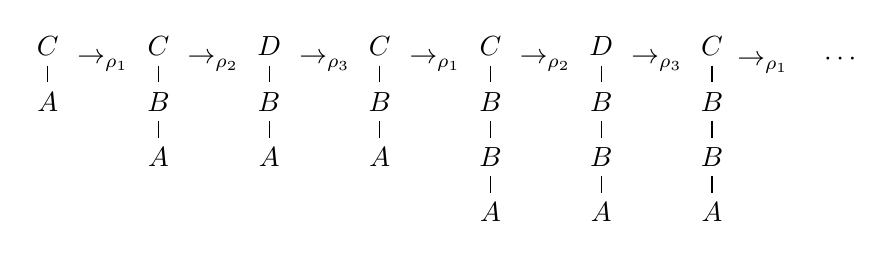
\begin{tikzpicture}[node distance=40pt]
\tikzstyle{level}=[level distance=20pt,sibling distance=22pt]
\node (a) {$C$} child { node {$A$} };
\node (a') [right of=a] {$C$} child { node {$B$} child { node {$A$} } };
\node (a'') [right of=a'] {$D$} child { node {$B$} child { node {$A$} } };
\node (b) [right of=a''] {$C$} child { node {$B$} child { node {$A$} } };
\node (b') [right of=b] {$C$} child { node {$B$} child { node {$B$}
    child { node {$A$} } } };
\node (b'') [right of=b'] {$D$} child { node {$B$} child { node {$B$}
    child { node {$A$} } } };
\node (c) [right of=b''] {$C$} child { node {$B$} child { node {$B$}
    child { node {$A$} } } };
\node (d) [right of=c] {};
\path (a) -- (a') node[midway,below=-1pt] {$\rightarrow_{\rho_1}$};
\path (a') -- (a'') node[midway,below=-1pt] {$\rightarrow_{\rho_2}$};
\path (a'') -- (b) node[midway,below=-1pt] {$\rightarrow_{\rho_3}$};
\path (b) -- (b') node[midway,below=-1pt] {$\rightarrow_{\rho_1}$};
\path (b') -- (b'') node[midway,below=-1pt] {$\rightarrow_{\rho_2}$};
\path (b'') -- (c) node[midway,below=-1pt] {$\rightarrow_{\rho_3}$};
\path (c) -- (d) node[pos=.8,below=-1pt] {$\rightarrow_{\rho_1} \quad \cdots$};
\end{tikzpicture}}
\end{center}\vspace{-0.8\baselineskip}
We can define this rewrite sequence as the limit of
$(\varphi_n)_{n \in \mathbb{N}}$, where $\concat$ denotes
concatenation of rewrite sequences:
\begin{align*}
  \varphi_0 \, &: \, C(A) \to^0 C(A)\\ % or \mbox{\emph{empty}}
  \varphi_{n + 1} \, &: \, \varphi_n \concat C(B^n(A)) \to_{\rho_1}
  C(B^{n + 1}(A)) \to_{\rho_2} D(B^{n + 1}(A)) \to_{\rho_3} C(B^{n +
    1}(A))
\end{align*}
The target terms $C(B^{n + 1}(A))$ converge to $C(B^\omega)$ and this
construction can thus be used with our inductive definition of rewrite
sequences, where we take $\varphi_n$ to be the $n$\textsuperscript{th}
branch of the \coqref{Rewriting.Lim}{\coqdocconstructor{Lim}}
constructor.

% $\varphi_n$ is the prefix of length $3n$.

% 'stuttering convergence'
% convergence with hiccups
% the difference between t_n and the limit t is oscillating

It is not clear to us whether there is some natural translation of the
convergence conditions to our formalisation.
%Without such a translation, we feel our definitions are not
%satisfactory.
For completeness we include a (not so natural) translation of
convergence, but we were not able to use it in our development. Even
proving the simplest convergent rewrite sequences to satisfy these
definitions seems too involved.
% TODO: try with the really simplest example and explain better why it doesn't
% work for us
\begin{singlespace}
\begin{coqdoccode}
\coqdocnoindent
\coqdockw{Fixpoint}
\coqdef{Rewriting.weaklyconvergent}{weakly\_convergent}{\coqdocdefinition{weakly\_convergent}}
\coqdocvar{s} \coqdocvar{t} (\coqdocvar{$\varphi$} : \coqdocvar{s}
\coqref{Rewriting.sequence}{$\rewrites_\mathcal{R}$} \coqdocvar{t}) :
\coqdockw{Prop}
:=\coqdoceol
\coqdocindent{1.00em}
\coqdockw{match} \coqdocvariable{$\varphi$} \coqdockw{with}\coqdoceol
\coqdocindent{1.00em}
\ensuremath{|} \coqref{Rewriting.Nil}{\coqdocconstructor{Nil}}
\coqdocvar{\_}          \ensuremath{\Rightarrow}
\coqexternalref{http://coq.inria.fr/stdlib/Coq.Init.Logic}{True}{\coqdocinductive{True}}\coqdoceol
\coqdocindent{1.00em}
\ensuremath{|} \coqref{Rewriting.Cons}{\coqdocconstructor{Cons}}
\coqdocvar{\_} \coqdocvar{\_} \coqdocvar{$\psi$} \coqdocvar{\_}
\coqdocvar{\_} \ensuremath{\Rightarrow}
\coqref{Rewriting.weaklyconvergent}{\coqdocdefinition{weakly\_convergent}}
\coqdocvariable{$\psi$}\coqdoceol
\coqdocindent{1.00em}
\ensuremath{|} \coqref{Rewriting.Lim}{\coqdocconstructor{Lim}}
\coqdocvar{\_} \coqdocvar{\_} \coqdocvar{f} \coqdocvar{t}
\coqdocvar{\_}  \ensuremath{\Rightarrow}
(\ensuremath{\forall} \coqdocvar{n},
\coqref{Rewriting.weaklyconvergent}{\coqdocdefinition{weakly\_convergent}}
(\coqdocvariable{f} \coqdocvariable{n})) \ensuremath{\land}\coqdoceol
\coqdocindent{2.00em}
\ensuremath{\forall} \coqdocvar{d}, \ensuremath{\exists}
\coqdocvar{$\iota$}, \ensuremath{\forall} \coqdocvar{$\kappa$},\coqdoceol
\coqdocindent{3.00em}
\coqdocvariable{$\varphi$}[\coqdocvariable{$\iota$}]$^\textsc{seq}$ \coqref{Rewriting.embed}{$\sqsubseteq$}
\coqdocvariable{$\varphi$}[\coqdocvariable{$\kappa$}]$^\textsc{seq}$
\ensuremath{\rightarrow}
\coqdocvariable{$\varphi$}[\coqdocvariable{$\kappa$}]$^\textsc{l}$
\coqref{TermEquality.termequpto}{\equpto{\coqdocvariable{d}}}
\coqdocvariable{t}\coqdoceol
\coqdocindent{1.00em}
\coqdockw{end}.\coqdoceol
\coqdocemptyline
\coqdocnoindent
\coqdockw{Fixpoint}
\coqdef{Rewriting.stronglyconvergent}{strongly\_convergent}{\coqdocdefinition{strongly\_convergent}}
\coqdocvar{s} \coqdocvar{t} (\coqdocvar{$\varphi$} : \coqdocvar{s} \coqref{Rewriting.sequence}{$\rewrites_\mathcal{R}$} \coqdocvar{t}) : \coqdockw{Prop}
:=\coqdoceol
\coqdocindent{1.00em}
\coqdockw{match} \coqdocvariable{$\varphi$} \coqdockw{with}\coqdoceol
\coqdocindent{1.00em}
\ensuremath{|} \coqref{Rewriting.Nil}{\coqdocconstructor{Nil}}
\coqdocvar{\_}          \ensuremath{\Rightarrow}
\coqexternalref{http://coq.inria.fr/stdlib/Coq.Init.Logic}{True}{\coqdocinductive{True}}\coqdoceol
\coqdocindent{1.00em}
\ensuremath{|} \coqref{Rewriting.Cons}{\coqdocconstructor{Cons}}
\coqdocvar{\_} \coqdocvar{\_} \coqdocvar{$\psi$} \coqdocvar{\_}
\coqdocvar{\_} \ensuremath{\Rightarrow}
\coqref{Rewriting.stronglyconvergent}{\coqdocdefinition{strongly\_convergent}}
\coqdocvariable{$\psi$}\coqdoceol
\coqdocindent{1.00em}
\ensuremath{|} \coqref{Rewriting.Lim}{\coqdocconstructor{Lim}}
\coqdocvar{\_} \coqdocvar{\_} \coqdocvar{f} \coqdocvar{t}
\coqdocvar{\_}  \ensuremath{\Rightarrow}
(\ensuremath{\forall} \coqdocvar{n},
\coqref{Rewriting.stronglyconvergent}{\coqdocdefinition{strongly\_convergent}}
(\coqdocvariable{f} \coqdocvariable{n})) \ensuremath{\land}\coqdoceol
\coqdocindent{2.00em}
\ensuremath{\forall} \coqdocvar{d}, \ensuremath{\exists}
\coqdocvar{$\iota$}, \ensuremath{\forall} \coqdocvar{$\kappa$},\coqdoceol
\coqdocindent{3.00em}
\coqdocvariable{$\varphi$}[\coqdocvariable{$\iota$}]$^\textsc{seq}$
\coqref{Rewriting.embed}{$\sqsubseteq$}
\coqdocvariable{$\varphi$}[\coqdocvariable{$\kappa$}]$^\textsc{seq}$
\ensuremath{\rightarrow}
\coqdocvariable{d} $\le$
\coqdocdefinition{depth}
\coqdocvariable{$\varphi$}[\coqdocvariable{$\kappa$}]$^\textsc{stp}$\coqdoceol
\coqdocindent{1.00em}
\coqdockw{end}.\coqdoceol
\end{coqdoccode}
\end{singlespace}

%Here it should be possible to prove that
%\coqref{Rewriting.stronglyconvergent}{\coqdocdefinition{strongly\_convergent}}
%implies
%\coqref{Rewriting.weaklyconvergent}{\coqdocdefinition{weakly\_convergent}}.


\section{Design Decisions}\label{sec:design}

We describe a number of design decisions that we had to make during
implementation.

%Why \Coq?


\subsection{Coinductive Terms}

We define the type of infinite terms by coinduction. Another often
used definition of $\TerI$ is by partial functions from positions to
symbols. This definition is troublesome to translate to \Coq, which
admits no partial functions. It might be possible to circumvent this
restriction using option types, or by some other means, but we suspect
that the resulting notion of terms would not be elegant. Coinduction
is a native concept in \Coq and we use it as such. The consequence is, that in
defining infinite terms, we are restricted to definitions in guarded form, see
Section~\ref{sec:guardedness}.


\subsection{Positions}

The set of positions of a given term is a restricted list of natural
numbers. This could probably be translated to \Coq by encoding the
restriction in the type of positions. It would result in quite
complicated definitions, however, and therefore we choose for
\coqref{Term.subterm}{\coqdocdefinition{subterm}} and
\coqref{Context.dig}{\coqdocdefinition{dig}} to take any list of
natural numbers and return option types to distinguish between
existing and non-existing positions. This comes at the cost of having
to handle the option types with every call of
\coqref{Term.subterm}{\coqdocdefinition{subterm}} or
\coqref{Context.dig}{\coqdocdefinition{dig}}.


\subsection{Bisimilarity in Rewrite Steps}\label{sub:bissteps}

In the definition of rewrite steps (Section~\ref{sec:seq}), we include
bisimilarity conditions on the source and target terms. The reason is
that we cannot rely on \Coq's small Leibniz equality. For consider two
rewrite steps $s_1 \to s_2$ and $t_1 \to t_2$, where $s_2 \bis
t_1$. We should be able to construct the rewrite sequence consisting
of these two steps, but the fact that the target term of the first
and the source term of the second can be identified must be encoded
somewhere. There are two places to do this: in the
\coqref{Rewriting.Cons}{\coqdocconstructor{Cons}} constructor
for rewrite sequences, or in the definition of rewrite steps. We
choose the latter because it turns out to be technically more
elegant.


\subsection{One-Hole Contexts}\label{sub:contexts}

We know of two obvious ways to represent multi-hole contexts:
by the coinductive term datatype augmented with a constructor for
holes or by a function whose arguments represent holes.
Both are unsatisfactory. The first representation requires a dynamic
check on the number of holes and it admits contexts with infinitely
many holes. The second representation cannot guarantee
that each hole occurs exactly once and its type, encoding the number of
holes, cannot be generalised. \citet{lindley-08} presents a quite
involved solution based on a type-level difference encoding of natural
numbers. We bypass the problem by only considering one-hole contexts.


\section{Conclusions}

Our representation of transfinite rewrite sequences based on tree
ordinals is original work. While the representation is natural to
implement in \Coq, we are disappointed by not being able to come up
with a natural translation of convergence for this
representation. Without such a translation, we feel our definitions
are not satisfactory and we hope that future work can remedy this.

%For example, it is quite conceivable that other means of indexing our
%rewrite sequences can be defined. Alternatives to our embedding
%relation might also be possible.

% TODO: cite Ketema
In an alternative representation as partial functions from
ordinals to rewrite steps, convergence can be expresssed directly, but it has
other problems. However, it seems
worthwhile to also investigate this representation further, for example
using the ordinals in Cantor normal form by
\citet{casteran-06}. Jeroen Ketema showed by personal communication
that, assuming some decidable properties on the ordinal representation,
constructive formalisation of some of the infinitary rewriting theory is
possible.

Working with \Coq has been an overall pleasant experience. During this
development, our main disturbance was with the guardedness condition
on corecursive definitions. Sometimes unguarded but natural
definitions are easily seen to be productive yet not accepted by
\Coq. One could hope for future additions to \Coq in this area, for
example in the form of user-supplied productivity proofs for
corecursive definitions to be admitted.

% TODO: count number of lines
Still, the amount of work that is required for a formalisation like
this is disproportionally large. Especially the implementation of the
counterexample to UN$^\infty$ in weakly orthogonal systems from
Chapter~\ref{chap:unwo} takes only a page to formulate on paper, while
it took us some $2,000$ lines of \Coq code to formalise.

%Original goal was compression.

%Formalising transfinite objects is hard.
